\documentclass[11pt,a4paper]{article}

% ------------------------------------------------------------------
% Paquetes
% ------------------------------------------------------------------
\usepackage[utf8]{inputenc}
\IfFileExists{lmodern.sty}{\usepackage[T1]{fontenc}\usepackage{lmodern}}{}
\IfFileExists{spanish.ldf}{%
  \usepackage[spanish,es-noshorthands,es-tabla]{babel}%
}{%
  \renewcommand{\contentsname}{Índice}%
  \renewcommand{\figurename}{Figura}%
  \renewcommand{\tablename}{Tabla}%
  \renewcommand{\refname}{Referencias}%
  \hyphenpenalty=10000 \exhyphenpenalty=10000%
}
\usepackage[a4paper,margin=2.5cm,headheight=14pt]{geometry}
\usepackage{amsmath,amssymb,amsthm,mathtools,bm}
\usepackage{xcolor}
\usepackage{booktabs,array}
\usepackage{graphicx}
\usepackage{float}
\usepackage{enumitem}
\usepackage{caption}
\usepackage{titlesec}
\usepackage{fancyhdr}
\usepackage{tikz}
\usepackage{pgfplots}
\pgfplotsset{compat=1.16}
\usepackage{algorithm}
\usepackage{algpseudocode}
\usepackage[hidelinks]{hyperref}

\emergencystretch=3em
\setlist{itemsep=2pt,topsep=4pt}
\setlength{\parskip}{5pt}
\setlength{\parindent}{0pt}
\linespread{1.08}

% ------------------------------------------------------------------
% Estilo sobrio: un solo color de acento
% ------------------------------------------------------------------
\definecolor{acento}{RGB}{0,95,105}
\captionsetup{font=small,labelfont={bf,color=acento},labelsep=period}

\pagestyle{fancy}
\fancyhf{}
\fancyhead[L]{\footnotesize Regresión Lineal Regularizada: Ridge y Elastic Net}
\fancyhead[R]{\footnotesize Optimización --- UTEC 2026}
\fancyfoot[C]{\footnotesize\thepage}
\renewcommand{\headrulewidth}{0.3pt}

\titleformat{\section}{\Large\bfseries\color{acento}}{\thesection}{0.6em}{}
\titlespacing*{\section}{0pt}{18pt}{6pt}
\titleformat{\subsection}{\large\bfseries}{\thesubsection}{0.6em}{}
\titlespacing*{\subsection}{0pt}{12pt}{4pt}

% Nota de cierre de cada modelo
\newcommand{\resumen}[1]{\par\medskip\noindent\textbf{\color{acento}En resumen:} #1\par\medskip}

% ------------------------------------------------------------------
% Macros
% ------------------------------------------------------------------
\newcommand{\R}{\mathbb{R}}
\newcommand{\norm}[1]{\left\lVert #1 \right\rVert}
\newcommand{\bt}{\bm{\beta}}
\newcommand{\bh}{\hat{\bm{\beta}}}
\DeclareMathOperator*{\argmin}{arg\,min}
\DeclareMathOperator{\sign}{sign}
\DeclareMathOperator{\tr}{tr}
\newcommand{\soft}{\mathcal{S}}
\newcolumntype{L}[1]{>{\raggedright\arraybackslash}p{#1}}

\newtheoremstyle{simple}{8pt}{8pt}{\itshape}{}{\bfseries\color{acento}}{.}{0.5em}{}
\theoremstyle{simple}
\newtheorem{proposicion}{Proposición}[section]

\floatname{algorithm}{Algoritmo}
\algrenewcommand\algorithmicrequire{\textbf{Entrada:}}
\algrenewcommand\algorithmicensure{\textbf{Salida:}}
\algrenewcommand\algorithmicfor{\textbf{para}}
\algrenewcommand\algorithmicdo{\textbf{hacer}}
\algrenewcommand\algorithmicend{\textbf{fin}}
\algrenewcommand\algorithmicrepeat{\textbf{repetir}}
\algrenewcommand\algorithmicuntil{\textbf{hasta que}}

\begin{document}

% ------------------------------------------------------------------
% Portada simple
% ------------------------------------------------------------------
\begin{center}
{\LARGE\bfseries\color{acento} Regresión Lineal Regularizada}\\[6pt]
{\Large Ridge y Elastic Net: fundamentos teóricos y algoritmos de optimización}\\[10pt]
{\large Proyecto P1 Optimización --- UTEC 2026 \\[2pt] Segunda entrega: validación empírica y usos profesionales}\\[4pt]
\textbf{Dataset:} precios de alquiler de inmuebles en Lima, Perú (elaboración propia a partir de Properati Perú, $n=720$, $p=34$)\\[8pt]
Cuevas Sánchez, Jorge \quad [202510326]\\[0pt]
Veramendi Hilario, Lando \quad [202210370]\\[0pt]
Murillo Chancahuaña, José Martín \quad [202510230]\\[0pt]
Cabanillas Solís, Joseph Jossemy \quad [202410347]\\[0pt]
Honores Chiroque, Flavia Marife \quad [202310550]
\end{center}
\vspace{2pt}\hrule\vspace{6pt}

% ==================================================================
\section{Introducción}
% ==================================================================
La regresión lineal múltiple aproxima una variable objetivo $y\in\R^n$ mediante una combinación lineal de predictores $X\in\R^{n\times p}$:
\begin{equation}
\hat y=\beta_0\mathbf 1+X\bt ,
\end{equation}
donde $\beta_0$ es el intercepto y $\bt=(\beta_1,\dots,\beta_p)^\top$ son los coeficientes. Los Mínimos Cuadrados Ordinarios (MCO) minimizan el error cuadrático sin restricciones. Funcionan bien con muchas observaciones y pocas variables independientes, pero fallan si hay muchos predictores o si están correlacionados: los coeficientes se vuelven inestables y el modelo sobreajusta. Si $p>n$, ni siquiera hay solución única.

La \emph{regularización} corrige esto sumando a la función de error una penalización sobre los coeficientes. Este trabajo estudia dos modelos:
\begin{itemize}
\item \textbf{Ridge} (Hoerl y Kennard, 1970 \cite{hoerl1970}): penalización L2, que contrae los coeficientes hacia cero sin anularlos.
\item \textbf{Elastic Net} (Zou y Hastie, 2005 \cite{zou2005}): mezcla de penalizaciones L1 y L2, que además de contraer puede anular coeficientes (selección de variables) y mantiene un comportamiento estable con variables correlacionadas.
\end{itemize}
Cada modelo se analiza desde la optimización: su función de error, el algoritmo que la minimiza, la interpretación de sus parámetros e hiperparámetros y sus fortalezas y desventajas. Cada uno incluye un ejemplo numérico resuelto a mano. Además, ambos algoritmos se implementan desde cero y se validan sobre un dataset realista de precios de alquiler (Sección~\ref{sec:dataset}), y se documentan sus usos actuales en el ámbito profesional (Sección~\ref{sec:usos}).

\paragraph{Notación.} Hay $n$ observaciones y $p$ variables; $X$ tiene columnas $x_1,\dots,x_p$. $\norm{\cdot}$ es la norma euclidiana y $\norm{\cdot}_1$ la norma $\ell_1$. Los valores singulares de $X$ son $s_1\ge\dots\ge s_p\ge0$. Salvo indicación contraria, $X$ y $y$ están \emph{centrados} (el intercepto se omite y se recupera después) y las columnas están \emph{estandarizadas} ($\norm{x_j}^2=n$), para que la penalización trate igual a todas las variables. Las funciones objetivo se escriben sin el factor $1/n$; la Sección~\ref{sec:sklearn} da la equivalencia con scikit-learn.

% ==================================================================
\section{Planteamiento del problema y objetivos}
% ==================================================================
\textbf{Problema.} Con variables numerosas, redundantes o correlacionadas, MCO da coeficientes inestables y poca capacidad de generalización. La regularización cambia el problema de optimización: en lugar de minimizar solo el error cuadrático, se minimiza el error más una penalización sobre $\bt$.

\textbf{Pregunta guía.} ¿Cómo se plantea y se resuelve el problema de optimización de Ridge y de Elastic Net, y cómo se interpretan sus coeficientes e hiperparámetros?

\textbf{Objetivo general.} Estudiar e implementar los modelos Ridge y Elastic Net, desde su formulación matemática hasta su validación con un dataset realista.

\textbf{Objetivos específicos.}
\begin{itemize}
\item Formular la función objetivo de cada modelo y analizar su convexidad y la unicidad de su solución.
\item Estudiar los algoritmos de minimización (solución cerrada, descenso del gradiente y descenso por coordenadas) y su convergencia.
\item Interpretar los coeficientes y los hiperparámetros ($\lambda$, $\alpha$) y describir su selección por validación cruzada.
\item Identificar las fortalezas y desventajas de cada modelo.
\item Implementar los algoritmos desde cero, validarlos contra scikit-learn y aplicarlos a un dataset realista.
\item Documentar los usos actuales de cada modelo en el ámbito profesional.
\end{itemize}
Esta entrega cubre los seis objetivos.

% ==================================================================
\section{Ridge}\label{sec:ridge}
% ==================================================================

\subsection{Idea y función objetivo}
MCO minimiza $f(\bt)=\tfrac12\norm{y-X\bt}^2$, cuyo gradiente es $\nabla f(\bt)=X^\top(X\bt-y)$. Sus condiciones de optimalidad son las \emph{ecuaciones normales} $X^\top X\bt=X^\top y$. Si existen direcciones con valor singular pequeño (multicolinealidad), la varianza del estimador crece como $\sigma^2\sum_j s_j^{-2}$, aunque MCO sea insesgado. Ridge añade una penalización L2 que introduce un pequeño sesgo a cambio de reducir esa varianza:
\begin{equation}\label{eq:PR}
\min_{\bt\in\R^p}\; F_R(\bt)=\tfrac12\norm{y-X\bt}^2+\tfrac{\lambda}{2}\norm{\bt}^2,\qquad \lambda\ge0 .
\end{equation}
El parámetro $\lambda$ controla el peso de la penalización, y el intercepto no se penaliza. Equivalentemente, se minimiza el error sujeto a $\norm{\bt}^2\le t$: la solución es el punto donde las elipses de nivel del error tocan una bola, que no tiene esquinas, por lo que ningún coeficiente se anula. Desde el punto de vista bayesiano, Ridge es la estimación máximo a posteriori con un prior gaussiano $\beta_j\sim\mathcal N(0,\tau^2)$, con $\lambda=\sigma^2/\tau^2$.

\begin{proposicion}[Convexidad]\label{prop:convR}
$F_R$ es fuertemente convexa para todo $\lambda>0$, con hessiano $X^\top X+\lambda I$. Su parámetro de convexidad es $\mu=s_p^2+\lambda$, la constante de Lipschitz de su gradiente es $L=s_1^2+\lambda$ y su número de condición es $\kappa(\lambda)=\frac{s_1^2+\lambda}{s_p^2+\lambda}$, que decrece al aumentar $\lambda$.
\end{proposicion}
\begin{proof}
Los autovalores de $X^\top X$ están en $[s_p^2,s_1^2]$, así que los de $X^\top X+\lambda I$ están en $[s_p^2+\lambda,\,s_1^2+\lambda]$. La derivada de $\lambda\mapsto\frac{a+\lambda}{b+\lambda}$ es $\frac{b-a}{(b+\lambda)^2}<0$ si $a>b$.
\end{proof}
Por tanto, el problema es convexo y suave: tiene un único mínimo, que es global.

\subsection{Solución cerrada}
Igualando el gradiente $X^\top(X\bt-y)+\lambda\bt$ a cero se obtiene $(X^\top X+\lambda I)\bt=X^\top y$. La matriz es definida positiva, luego invertible:
\begin{equation}
\bh_R(\lambda)=(X^\top X+\lambda I)^{-1}X^\top y=\sum_{j}\frac{s_j}{s_j^2+\lambda}\,(u_j^\top y)\,v_j ,
\end{equation}
donde $X=\sum_j s_j u_j v_j^\top$ es la descomposición en valores singulares. Frente a MCO, cada componente se multiplica por el factor de contracción $\frac{s_j^2}{s_j^2+\lambda}\in(0,1)$: las direcciones con valor singular pequeño, responsables de la varianza excesiva, son las más contraídas. La solución existe y es única incluso si $p>n$.

\emph{Costo.} Formar $X^\top X$ cuesta $O(np^2)$ y su factorización de Cholesky $O(p^3)$. Para $p$ grande esto es caro y conviene un método iterativo.

\subsection{Descenso del gradiente}
La iteración es
\begin{equation}\label{eq:gd}
\bt_{k+1}=\bt_k-\eta\big[X^\top(X\bt_k-y)+\lambda\bt_k\big].
\end{equation}
\begin{proposicion}[Convergencia lineal]\label{prop:gd}
Con $\mu$, $L$ y $\kappa=L/\mu$ como en la Proposición~\ref{prop:convR} y paso $\eta=1/L$,
\[
\norm{\bt_k-\bh_R}\le\Big(1-\frac1\kappa\Big)^{k}\norm{\bt_0-\bh_R}.
\]
\end{proposicion}
\begin{proof}
Como $F_R$ es cuadrática, $\nabla F_R(\bt)=H(\bt-\bh_R)$ con $H=X^\top X+\lambda I$, y entonces $\bt_{k+1}-\bh_R=(I-\eta H)(\bt_k-\bh_R)$. Con $\eta=1/L$, los autovalores de $I-\eta H$ están en $[0,\,1-\mu/L]$. Se concluye con la norma espectral.
\end{proof}
Se necesitan del orden de $\kappa\log(1/\varepsilon)$ iteraciones para una precisión $\varepsilon$, y cada una cuesta $O(np)$. Como $\kappa$ decrece con $\lambda$, la regularización cumple un doble papel: reduce la varianza y mejora el condicionamiento numérico.

\subsection{Ejemplo numérico}
Sea $n=3$, $p=2$, sin intercepto, y $\lambda=1$:
\[
X=\begin{pmatrix}1&1\\1&0\\0&1\end{pmatrix},\qquad y=\begin{pmatrix}3\\1\\2\end{pmatrix}.
\]
\textbf{MCO.} $X^\top X=\begin{pmatrix}2&1\\1&2\end{pmatrix}$ y $X^\top y=(4,5)^\top$, de donde $\bh_{\mathrm{MCO}}=(1,2)^\top$.

\textbf{Solución cerrada.} $X^\top X+\lambda I=\begin{pmatrix}3&1\\1&3\end{pmatrix}$, con inversa $\tfrac18\begin{pmatrix}3&-1\\-1&3\end{pmatrix}$. Entonces
\[
\bh_R=\tfrac18\begin{pmatrix}3\cdot4-5\\-4+3\cdot5\end{pmatrix}=\begin{pmatrix}7/8\\11/8\end{pmatrix}=\begin{pmatrix}0.875\\1.375\end{pmatrix}.
\]
Los autovalores de $X^\top X$ son $3$ y $1$, así que los factores de contracción $s_j^2/(s_j^2+\lambda)$ valen $3/4$ y $1/2$: la dirección más débil se contrae más.

\textbf{Descenso del gradiente.} Aquí $L=4$, $\mu=2$ y $\kappa=2$; se usa $\eta=1/4$ y $\bt_0=(0,0)^\top$.
\begin{itemize}
\item Iteración 1: el gradiente en $\bt_0$ es $(-4,-5)^\top$, luego $\bt_1=(1,\,1.25)^\top$.
\item Iteración 2: el gradiente en $\bt_1$ es $\begin{pmatrix}3&1\\1&3\end{pmatrix}\!\begin{pmatrix}1\\1.25\end{pmatrix}-\begin{pmatrix}4\\5\end{pmatrix}=\begin{pmatrix}0.25\\-0.25\end{pmatrix}$, luego $\bt_2=(0.9375,\,1.3125)^\top$.
\end{itemize}
Los errores $\norm{\bt_k-\bh_R}$ son $0.1768$ y $0.0884$: se reducen a la mitad en cada iteración, en línea con la cota $(1-1/\kappa)^k=0.5^k$.

\subsection{Interpretación de coeficientes e hiperparámetro}
\textbf{Coeficientes.} Con variables estandarizadas, $\hat\beta_j$ es el cambio esperado en la respuesta por cada desviación estándar de $x_j$, manteniendo las demás fijas. Es una asociación, no una relación causal, y como están contraídos hacia cero, subestiman el efecto real. En Ridge todos los coeficientes son distintos de cero, y cuando dos variables están muy correlacionadas el peso se reparte entre ellas de forma estable.

\textbf{El hiperparámetro $\lambda$.} Regula la contracción y con ella la complejidad del modelo:
\begin{itemize}
\item Si $\lambda\to0^+$, Ridge se acerca a MCO; si $\lambda\to\infty$, los coeficientes tienden a $0$ de forma continua.
\item Los grados de libertad efectivos son $\mathrm{df}(\lambda)=\sum_j\frac{s_j^2}{s_j^2+\lambda}$, que decrece de $p$ (si $\operatorname{rango}(X)=p$) a $0$.
\item $\lambda$ pequeño da bajo sesgo y alta varianza (sobreajuste); $\lambda$ grande da alto sesgo y baja varianza (subajuste). El error de validación suele tener forma de U.
\end{itemize}

\textbf{Selección por validación cruzada.}\label{sec:cv} Los hiperparámetros no se ajustan con los mismos datos que los coeficientes. El procedimiento estándar es la validación cruzada de $K$ pliegues ($K=5$ o $10$):
\begin{enumerate}
\item Definir una grilla de valores de $\lambda$ en escala logarítmica.
\item Para cada pliegue, ajustar el modelo con los datos de entrenamiento (el preprocesamiento se calcula solo con ellos, para evitar fuga de información) y medir el error en el pliegue de validación.
\item Elegir el $\lambda$ de menor error medio o, alternativamente, el mayor $\lambda$ cuyo error esté a una desviación estándar del mínimo, que favorece modelos más simples \cite{hastie2009}.
\end{enumerate}
Los algoritmos iterativos tienen además sus propios parámetros (paso $\eta$, tolerancia, iteraciones máximas), que afectan la precisión numérica pero no la definición del modelo.

\subsection{Fortalezas y desventajas}
\textbf{Fortalezas:}
\begin{itemize}
\item Estabiliza la estimación ante multicolinealidad y funciona cuando $p>n$.
\item Tiene solución cerrada; el gradiente converge linealmente.
\item Un solo hiperparámetro ($\lambda$).
\item Mejora el condicionamiento numérico y reduce la varianza de las predicciones.
\end{itemize}
\textbf{Desventajas:}
\begin{itemize}
\item No produce ceros exactos: no selecciona variables y el modelo conserva los $p$ predictores.
\item La contracción sesga los coeficientes, lo que complica la inferencia.
\item Requiere estandarizar los predictores.
\item Con $p$ grande, es difícil de interpretar porque ningún coeficiente se elimina.
\end{itemize}

\resumen{la penalización L2 vuelve el problema fuertemente convexo, con solución cerrada y convergencia lineal del gradiente, que mejora al aumentar $\lambda$. Estabiliza el modelo ante variables correlacionadas, pero no selecciona variables.}

% ==================================================================
\section{Elastic Net}\label{sec:en}
% ==================================================================

\subsection{Idea y función objetivo}
Elastic Net combina las penalizaciones L1 y L2 con dos hiperparámetros: $\lambda\ge0$, que controla la intensidad total, y $\alpha\in[0,1]$, que fija la proporción de L1:
\begin{equation}\label{eq:PE}
\min_{\bt\in\R^p}\; F_E(\bt)=\tfrac12\norm{y-X\bt}^2+\lambda\Big[\alpha\norm{\bt}_1+\tfrac{1-\alpha}{2}\norm{\bt}_2^2\Big].
\end{equation}
El término L1 puede llevar coeficientes \emph{exactamente} a cero, lo que da selección automática de variables. El término L2 estabiliza la solución. Con $\alpha=1$ solo queda L1 y con $\alpha=0$ solo L2, que es Ridge. Geométricamente, la región factible tiene esquinas sobre los ejes (que permiten ceros) y bordes curvos.

Elastic Net tiene además el \emph{efecto de agrupación}: cuando varias variables están correlacionadas, tiende a asignarles coeficientes similares y a mantenerlas o eliminarlas juntas \cite{zou2005}. Aquí no se aplica el reescalado por $(1+\lambda_2)$ que proponen Zou y Hastie, igual que en scikit-learn y \texttt{glmnet}. Bayesianamente, la penalización corresponde a un prior que combina el gaussiano y el de Laplace.

\begin{proposicion}[Convexidad y unicidad]\label{prop:convE}
$F_E$ es convexa y coerciva. Si $\alpha<1$, es fuertemente convexa con parámetro al menos $\lambda(1-\alpha)$, y por tanto tiene un único minimizador, incluso cuando $p>n$.
\end{proposicion}
\begin{proof}
$F_E$ es la suma de $\tfrac12\norm{y-X\bt}^2+\lambda\alpha\norm{\bt}_1$, que es convexa, y de $\tfrac{\lambda(1-\alpha)}{2}\norm{\bt}^2$, que es fuertemente convexa con parámetro $\lambda(1-\alpha)$.
\end{proof}

\subsection{Optimalidad y umbralización suave}
La norma $\ell_1$ no es diferenciable en $\beta_j=0$, así que no hay una solución cerrada. Su subdiferencial es $\{\sign(\beta_j)\}$ si $\beta_j\ne0$ y $[-1,1]$ si $\beta_j=0$. Con el residuo $r=y-X\bh$, las condiciones de optimalidad de Elastic Net son
\begin{equation}\label{eq:kkt}
\begin{cases}
x_j^\top r-\lambda(1-\alpha)\hat\beta_j=\lambda\alpha\,\sign(\hat\beta_j) & \text{si } \hat\beta_j\ne0,\\[2pt]
|x_j^\top r|\le\lambda\alpha & \text{si } \hat\beta_j=0.
\end{cases}
\end{equation}
La segunda línea explica por qué se eliminan variables: si la correlación de $x_j$ con el residuo no supera el umbral $\lambda\alpha$, el valor $\hat\beta_j=0$ es óptimo. En particular, $\bh=0$ si y solo si $\lambda\alpha\ge\norm{X^\top y}_\infty$, lo que da el punto de partida de la grilla de $\lambda$.

La solución de subproblemas de una variable usa el operador de \emph{umbralización suave}:
\begin{equation}\label{eq:soft}
\soft_\tau(z)=\sign(z)\max\{|z|-\tau,0\}=\begin{cases}z-\tau,& z>\tau,\\ z+\tau,& z<-\tau,\\ 0,& |z|\le\tau,\end{cases}
\end{equation}
que resta $\tau$ al valor absoluto y anula todo lo que no lo supera (Figura~\ref{fig:soft}).

\begin{figure}[H]
\centering
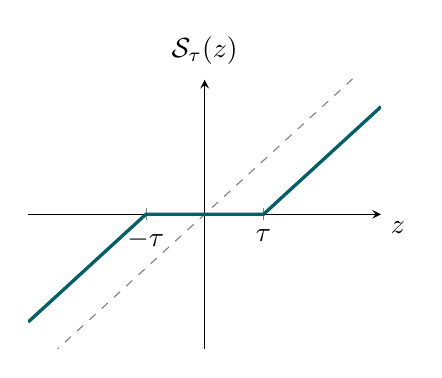
\begin{tikzpicture}
\begin{axis}[
  width=0.5\textwidth,height=5cm,
  axis lines=middle,
  xmin=-3,xmax=3,ymin=-2.5,ymax=2.5,
  xlabel={$z$}, ylabel={$\soft_\tau(z)$},
  xlabel style={at={(axis description cs:1,0.45)},anchor=west},
  ylabel style={at={(axis description cs:0.5,1.02)},anchor=south},
  xtick={-1,1}, xticklabels={$-\tau$,$\tau$}, ytick=\empty]
\addplot[dashed,gray] coordinates {(-3,-3) (3,3)};
\addplot[acento,very thick] coordinates {(-3,-2) (-1,0) (1,0) (3,2)};
\end{axis}
\end{tikzpicture}
\caption{Umbralización suave (con $\tau=1$): la línea punteada es $y=z$.}
\label{fig:soft}
\end{figure}

\subsection{Descenso por coordenadas}
El método principal actualiza una coordenada $\beta_j$ a la vez, con las demás fijas. Con el residuo parcial $r_j=y-\sum_{l\ne j}x_l\beta_l$, el subproblema en $\beta_j$ tiene solución exacta
\begin{equation}\label{eq:cd-enet}
\beta_j\leftarrow\frac{\soft_{\lambda\alpha}(x_j^\top r_j)}{\norm{x_j}^2+\lambda(1-\alpha)} .
\end{equation}
El umbral $\lambda\alpha$ viene de la parte L1 y el término $\lambda(1-\alpha)$ del denominador, de la parte L2. Para $\alpha=0$ se recupera Ridge, $\beta_j\leftarrow x_j^\top r_j/(\norm{x_j}^2+\lambda)$. Manteniendo actualizado el residuo completo, cada actualización cuesta $O(n)$ y un ciclo completo $O(np)$.

\begin{algorithm}[ht]
\caption{Descenso por coordenadas para Elastic Net}\label{alg:cd}
\begin{algorithmic}[1]
\Require $X$, $y$, $\lambda>0$, $\alpha\in(0,1]$, punto inicial $\bt$, tolerancia $\mathrm{tol}$
\State $r\gets y-X\bt$
\Repeat
  \For{$j=1,\dots,p$}
    \State $z_j\gets x_j^\top r+\norm{x_j}^2\beta_j$
    \State $\beta_j^{\mathrm{nuevo}}\gets\soft_{\lambda\alpha}(z_j)\,/\,\big(\norm{x_j}^2+\lambda(1-\alpha)\big)$
    \State $r\gets r-x_j\,(\beta_j^{\mathrm{nuevo}}-\beta_j)$
    \State $\beta_j\gets\beta_j^{\mathrm{nuevo}}$
  \EndFor
\Until{el cambio máximo en $\bt$ es menor que $\mathrm{tol}$}
\Ensure $\bt$
\end{algorithmic}
\end{algorithm}

Aunque $F_E$ no es diferenciable, el método converge al óptimo porque la parte no suave es separable por coordenadas (Tseng \cite{tseng2001}). En la práctica se recorre una grilla decreciente de $\lambda$ usando la solución de cada valor como punto inicial del siguiente (\emph{warm start}), que es la base de \texttt{glmnet} \cite{friedman2010}.

\subsection{Alternativa: gradiente proximal (ISTA)}
Otra opción es tratar aparte la parte suave $f(\bt)=\tfrac12\norm{y-X\bt}^2+\tfrac{\lambda(1-\alpha)}{2}\norm{\bt}^2$, con constante de Lipschitz $L=s_1^2+\lambda(1-\alpha)$, y aplicar umbralización a la parte L1:
\begin{equation}\label{eq:ista}
\bt_{k+1}=\soft_{\lambda\alpha/L}\!\Big(\bt_k-\tfrac1L\big[X^\top(X\bt_k-y)+\lambda(1-\alpha)\bt_k\big]\Big).
\end{equation}
Es un paso de gradiente seguido de una umbralización, con costo $O(np)$ por iteración. Para $\alpha<1$ el problema es fuertemente convexo (Proposición~\ref{prop:convE}) y el método converge linealmente, con tasa $1-\mu/L$ y $\mu\ge\lambda(1-\alpha)$ \cite{beck2017}. Su versión acelerada, FISTA \cite{beck2009}, añade un paso de extrapolación y mejora la tasa sublineal de $O(1/k)$ a $O(1/k^2)$ en el caso general.

\subsection{Ejemplo numérico}
Con los mismos datos del ejemplo de Ridge ($\norm{x_1}^2=\norm{x_2}^2=2$, $X^\top y=(4,5)^\top$), sea $\lambda=1$ y $\alpha=0.5$. El umbral es $\lambda\alpha=0.5$ y el denominador es $2+\lambda(1-\alpha)=2.5$. Se aplica el Algoritmo~\ref{alg:cd} desde $\bt=(0,0)^\top$, con $r=y=(3,1,2)^\top$.

\textbf{Ciclo 1.}
\[
\begin{aligned}
&z_1=x_1^\top r=4,\quad \soft_{0.5}(4)=3.5\;\Rightarrow\;\beta_1=\tfrac{3.5}{2.5}=1.4,\quad r=(1.6,\,-0.4,\,2)^\top,\\
&z_2=x_2^\top r=3.6,\quad \soft_{0.5}(3.6)=3.1\;\Rightarrow\;\beta_2=\tfrac{3.1}{2.5}=1.24,\quad r=(0.36,\,-0.4,\,0.76)^\top.
\end{aligned}
\]
\textbf{Ciclo 2.}
\[
\begin{aligned}
&z_1=x_1^\top r+2\cdot1.4=2.76,\quad \soft_{0.5}(2.76)=2.26\;\Rightarrow\;\beta_1=0.904,\quad r=(0.856,\,0.096,\,0.76)^\top,\\
&z_2=(0.856+0.76)+2\cdot1.24=4.096,\quad \soft_{0.5}(4.096)=3.596\;\Rightarrow\;\beta_2=1.4384.
\end{aligned}
\]
El proceso continúa hasta que el cambio máximo sea menor que la tolerancia y converge a $\bh_{E}\approx(0.8095,\,1.4762)^\top$. Se verifica con las condiciones \eqref{eq:kkt}: al ser ambos coeficientes no nulos, $(X^\top X+0.5\,I)\bh=X^\top y-0.5\,\mathbf 1$, es decir,
\[
\begin{pmatrix}2.5&1\\1&2.5\end{pmatrix}\bh=\begin{pmatrix}3.5\\4.5\end{pmatrix}\;\Longrightarrow\;\bh=\tfrac{1}{5.25}\begin{pmatrix}2.5\cdot3.5-4.5\\2.5\cdot4.5-3.5\end{pmatrix}=\begin{pmatrix}0.8095\\1.4762\end{pmatrix}.
\]

\textbf{Un $\lambda$ mayor: eliminación de una variable.} Con $\lambda=8$ y $\alpha=0.5$, el umbral es $\lambda\alpha=4$ y el denominador $2+4=6$ (aquí $\bh=0$ ocurre si $\lambda\alpha\ge5$, es decir, $\lambda\ge10$). Desde $\bt=0$:
\[
z_1=4\le4\;\Rightarrow\;\beta_1=0;\qquad z_2=5,\;\soft_4(5)=1\;\Rightarrow\;\beta_2=\tfrac16\approx0.1667 .
\]
Un segundo ciclo no cambia nada, luego $\bh_E=(0,\,1/6)^\top$. Se cumplen las condiciones \eqref{eq:kkt}: para $j=1$, $x_1^\top r=4-\tfrac16=3.83\le4$, y para $j=2$, $x_2^\top r-4\cdot\tfrac16=4.667-0.667=4=\lambda\alpha$. El algoritmo no solo ajusta magnitudes: decide qué variables permanecen.

\subsection{Interpretación de coeficientes e hiperparámetros}
\textbf{Coeficientes.} Igual que en Ridge, con variables estandarizadas $\hat\beta_j$ es el cambio esperado en la respuesta por cada desviación estándar de $x_j$, con las demás fijas (asociación, no causalidad, y con sesgo hacia cero). Si $\hat\beta_j=0$, la variable fue descartada; si varias variables están muy correlacionadas, tienden a recibir coeficientes similares.

\textbf{Hiperparámetros.}
\begin{itemize}
\item $\lambda$: intensidad total de la penalización. Valores altos simplifican el modelo (más ceros); valores bajos permiten más complejidad.
\item $\alpha$: mezcla entre L1 y L2. Cerca de $1$ da modelos más ralos; cerca de $0$ da modelos más estables ante la correlación.
\item Ambos se eligen por validación cruzada (Sección~\ref{sec:ridge}) sobre una grilla bidimensional $(\lambda,\alpha)$.
\end{itemize}

\begin{table}[H]
\centering
\caption{Hiperparámetros de los modelos.}\label{tab:hiper}
\small
\begin{tabular}{@{}L{2.6cm}L{3.1cm}L{3.9cm}L{3.2cm}@{}}
\toprule
\textbf{Símbolo} & \textbf{Rol} & \textbf{Efecto al aumentarlo} & \textbf{Selección}\\
\midrule
$\lambda$ & Intensidad de la penalización & Más contracción y sesgo; menos varianza & Validación cruzada, grilla logarítmica\\
$\alpha$ & Mezcla L1/L2 (Elastic Net) & Más esparsidad, menos agrupación & Validación cruzada\\
$\eta$, tol, iter. máx. & Parámetros del algoritmo & Afectan velocidad y precisión & $\eta=1/L$; criterio de convergencia\\
\bottomrule
\end{tabular}
\end{table}

\subsection{Fortalezas y desventajas}
\textbf{Fortalezas:}
\begin{itemize}
\item Selecciona variables (vía L1) y mantiene estabilidad ante correlación (vía L2).
\item Efecto de agrupación: las variables correlacionadas se retienen o eliminan juntas.
\item Con $\alpha<1$, la solución es única aun con $p\gg n$ y no hay límite de $n$ variables activas.
\item Es flexible: incluye a Ridge ($\alpha=0$) como caso particular.
\end{itemize}
\textbf{Desventajas:}
\begin{itemize}
\item Tiene dos hiperparámetros ($\lambda$ y $\alpha$), lo que hace obligatoria la validación cruzada y multiplica su costo.
\item No tiene solución cerrada: requiere algoritmos iterativos.
\item La contracción sesga los coeficientes y hay que estandarizar los predictores.
\item Es un modelo lineal: no captura relaciones intrínsecamente no lineales.
\end{itemize}

\resumen{Elastic Net combina la selección de variables de L1 con la estabilidad de L2. Para $\alpha<1$ el problema es fuertemente convexo con solución única, y se resuelve con descenso por coordenadas o gradiente proximal usando un umbral $\lambda\alpha$ y un denominador ampliado por $\lambda(1-\alpha)$. Su costo es un hiperparámetro adicional.}

% ==================================================================
\section{Correspondencia con scikit-learn}\label{sec:sklearn}
% ==================================================================
Las funciones objetivo de este informe no incluyen el factor $1/n$, mientras que scikit-learn \cite{pedregosa2011} sí lo usa en Elastic Net. Para validar las implementaciones (Sección~\ref{sec:dataset}) conviene fijar la equivalencia (con \texttt{fit\_intercept=True}, que equivale a centrar los datos):

\begin{table}[H]
\centering
\caption{Equivalencia de parámetros con scikit-learn ($\alpha_{\mathrm{sk}}$ es su parámetro \texttt{alpha}).}\label{tab:sklearn}
\small
\renewcommand{\arraystretch}{1.4}
\begin{tabular}{@{}L{1.7cm}L{4.9cm}L{5.6cm}L{2.7cm}@{}}
\toprule
\textbf{Modelo} & \textbf{Este informe} & \textbf{scikit-learn} & \textbf{Equivalencia}\\
\midrule
Ridge & $\tfrac12\norm{y-X\bt}^2+\tfrac\lambda2\norm{\bt}^2$ & $\norm{y-Xw}^2+\alpha_{\mathrm{sk}}\norm{w}^2$ & $\lambda=\alpha_{\mathrm{sk}}$\\[4pt]
Elastic Net & $\tfrac12\norm{y-X\bt}^2+\lambda\big[\alpha\norm{\bt}_1+\tfrac{1-\alpha}2\norm{\bt}^2\big]$ & $\tfrac1{2n}\norm{y-Xw}^2+\alpha_{\mathrm{sk}}\rho\norm{w}_1+\tfrac{\alpha_{\mathrm{sk}}(1-\rho)}2\norm{w}^2$ & $\lambda=n\,\alpha_{\mathrm{sk}}$, $\alpha=\rho$ (\texttt{l1\_ratio})\\
\bottomrule
\end{tabular}
\end{table}

Con los datos de los ejemplos ($n=3$, \texttt{fit\_intercept=False}), se reproducen los cálculos a mano:
\begin{itemize}
\item \texttt{Ridge(alpha=1)} da $(0.875,\,1.375)$;
\item \texttt{ElasticNet(alpha=1/3, l1\_ratio=0.5)} da $(0.8095,\,1.4762)$.
\end{itemize}

% ==================================================================
\section{Validación con un dataset realista}\label{sec:dataset}
% ==================================================================
Se implementaron Ridge (solución cerrada, Sección~\ref{sec:ridge}) y Elastic Net (descenso por coordenadas, Algoritmo~\ref{alg:cd}) \emph{desde cero} en \texttt{NumPy}, y se validaron sobre un conjunto de datos real.

\subsection{El dataset}
Se construyó un dataset de \textbf{precios de alquiler de inmuebles en Lima, Perú}, a partir de $1079$ publicaciones extraídas del portal Properati Perú (anuncios activos entre octubre de 2022 y marzo de 2023). Cada fila original contenía texto semiestructurado (p. ej. \texttt{"S/.2,600"}, \texttt{"3 dormitorios"}, \texttt{"70 m²"}), por lo que se realizó un proceso de limpieza:
\begin{itemize}
\item \textbf{Precio:} se unificó a soles (\texttt{PEN}), convirtiendo los anuncios en dólares con un tipo de cambio de referencia (USD/PEN $\approx 3.80$).
\item \textbf{Dormitorios, baños y área:} se extrajeron como variables numéricas desde el texto libre.
\item \textbf{Año de construcción:} se convirtió a antigüedad (\texttt{age\_years}); los valores corruptos (celdas que contenían \texttt{"m²"} por error de captura del portal) se descartaron.
\item \textbf{Mantenimiento:} se extrajo el monto en soles; cuando no se publicaba, se usó $0$ junto con una variable indicadora \texttt{has\_maintenance}.
\item \textbf{Distrito:} se extrajo de la columna de ubicación; se conservaron como categorías los 11 distritos con al menos 15 anuncios, y el resto se agrupó en \texttt{Otro}.
\item \textbf{Filtros de calidad:} se restringió a \texttt{Apartamento} y \texttt{Casa} en el departamento de Lima, con precio entre S/.300 y S/.30\,000, área entre 15 y 1000 m\textsuperscript{2}, y hasta 10 dormitorios/baños, para excluir errores de digitación y anuncios atípicos (oficinas, locales comerciales, etc.).
\end{itemize}
Tras la limpieza quedaron $n=720$ observaciones completas (sin valores faltantes). La variable objetivo es el \textbf{logaritmo del precio}, porque la distribución del precio es muy asimétrica (coeficiente de asimetría $2.52$) y el logaritmo la corrige casi por completo ($0.11$); además, en un modelo log-lineal cada coeficiente se interpreta directamente como un efecto porcentual sobre el precio, lo cual es estándar en modelos hedónicos de precios inmobiliarios.

A partir de las $8$ variables base (dormitorios, baños, área, antigüedad, mantenimiento, tipo de inmueble y distrito) se construyó una matriz de diseño con $p=34$ predictores: las variables numéricas, variables \textit{dummy} de distrito y tipo de inmueble, interacciones relevantes (\texttt{area*distrito}, para capturar que el precio por m\textsuperscript{2} difiere por zona; \texttt{area*dormitorios}, \texttt{area*baños}, \texttt{dormitorios*baños}) y dos términos cuadráticos (\texttt{area\_m2\textsuperscript{2}}, \texttt{age\_years\textsuperscript{2}}) para capturar rendimientos decrecientes del tamaño y de la antigüedad. Como se esperaba, dormitorios, baños y área están fuertemente correlacionados entre sí (correlaciones de Pearson entre $0.56$ y $0.72$), y varias columnas de interacción comparten información con sus componentes: es exactamente el escenario de multicolinealidad que motiva Ridge y Elastic Net frente a MCO (Secciones~\ref{sec:ridge}--\ref{sec:en}).

\subsection{Protocolo experimental}
Se separó el $20\,\%$ de las observaciones como conjunto de prueba ($n_{\mathrm{test}}=144$) y el resto para entrenamiento ($n_{\mathrm{train}}=576$), con semilla aleatoria fija. Todas las variables se centraron y estandarizaron usando \emph{solo} las estadísticas del conjunto de entrenamiento, y esas mismas estadísticas se aplicaron al conjunto de prueba, para evitar fuga de información. El hiperparámetro de Ridge y el par $(\lambda,\alpha)$ de Elastic Net se eligieron por validación cruzada de $5$ pliegues sobre el conjunto de entrenamiento (Sección~\ref{sec:cv}), con una grilla logarítmica de $\lambda$ y, para Elastic Net, $\alpha\in\{0.1,0.3,0.5,0.7,0.9,1.0\}$.

\begin{table}[H]
\centering
\caption{Hiperparámetros óptimos por validación cruzada (5 pliegues).}\label{tab:hiper-opt}
\small
\begin{tabular}{@{}lll@{}}
\toprule
\textbf{Modelo} & \textbf{Hiperparámetros óptimos} & \textbf{MSE de validación cruzada}\\
\midrule
Ridge & $\lambda_{\min}=1.96$ (regla 1-SE: $\lambda_{1\text{SE}}=13.34$) & $0.0995$\\
Elastic Net & $\lambda^\star=0.70$, $\alpha^\star=0.9$ & $0.0985$\\
\bottomrule
\end{tabular}
\end{table}

La Figura~\ref{fig:cv-ridge} muestra la curva de validación cruzada de Ridge: el error decrece, alcanza un mínimo y vuelve a crecer para $\lambda$ grande, la forma de U característica del compromiso sesgo-varianza (Sección~\ref{sec:ridge}). Que la validación cruzada de Elastic Net elija $\alpha^\star=0.9$ (cercano a LASSO puro) con un $\lambda^\star$ moderado sugiere que casi todos los predictores aportan información, pero que un pequeño subconjunto es redundante dada la presencia de los demás.

\begin{figure}[H]
\centering
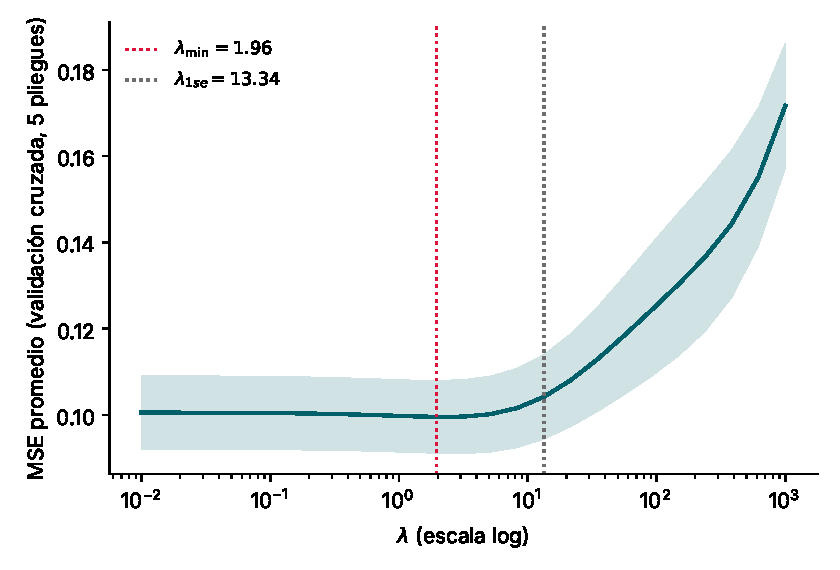
\includegraphics[width=0.62\textwidth]{figs/cv_ridge.pdf}
\caption{Validación cruzada de Ridge: MSE promedio (5 pliegues) en función de $\lambda$. La banda sombreada es $\pm 1$ error estándar.}
\label{fig:cv-ridge}
\end{figure}

\subsection{Resultados}
Con los hiperparámetros óptimos, ambos modelos se reentrenaron sobre todo el conjunto de entrenamiento y se evaluaron en el conjunto de prueba, nunca visto durante la validación cruzada (Tabla~\ref{tab:resultados}). Como referencia se incluye MCO sin regularizar ($\lambda\to0$).

\begin{table}[H]
\centering
\caption{Desempeño en el conjunto de prueba ($n_{\mathrm{test}}=144$), sobre $\log(\text{precio})$.}\label{tab:resultados}
\small
\begin{tabular}{@{}lcccc@{}}
\toprule
\textbf{Modelo} & $R^2$ & \textbf{RMSE} & \textbf{MAE} & \textbf{Error típico\footnotemark}\\
\midrule
MCO (sin regularizar) & $0.7839$ & $0.3171$ & $0.2366$ & $26.7\,\%$\\
Ridge ($\lambda=1.96$) & $0.7833$ & $0.3176$ & $0.2366$ & $26.7\,\%$\\
Elastic Net ($\lambda=0.70,\ \alpha=0.9$) & $\mathbf{0.7912}$ & $\mathbf{0.3117}$ & $\mathbf{0.2332}$ & $\mathbf{26.3\,\%}$\\
\bottomrule
\end{tabular}
\end{table}
\footnotetext{$\exp(\mathrm{MAE})-1$: error porcentual típico sobre el precio en soles.}

Elastic Net obtiene el mejor desempeño de los tres, superando incluso a MCO: con $p=34$ predictores correlacionados y solo $n_{\mathrm{train}}=576$ observaciones, la penalización reduce el sobreajuste sin sacrificar capacidad predictiva. Ridge, en cambio, queda prácticamente empatado con MCO en este dataset, porque $p\ll n$ y la multicolinealidad, aunque presente, no es tan severa como para que la contracción por sí sola aporte una mejora notable; su ventaja aparece sobre todo en la estabilidad de los coeficientes individuales (Sección~\ref{sec:interp-coef-datos}), no en el error agregado. La Figura~\ref{fig:pred-real} muestra las predicciones contra los valores reales en el conjunto de prueba.

\begin{figure}[H]
\centering
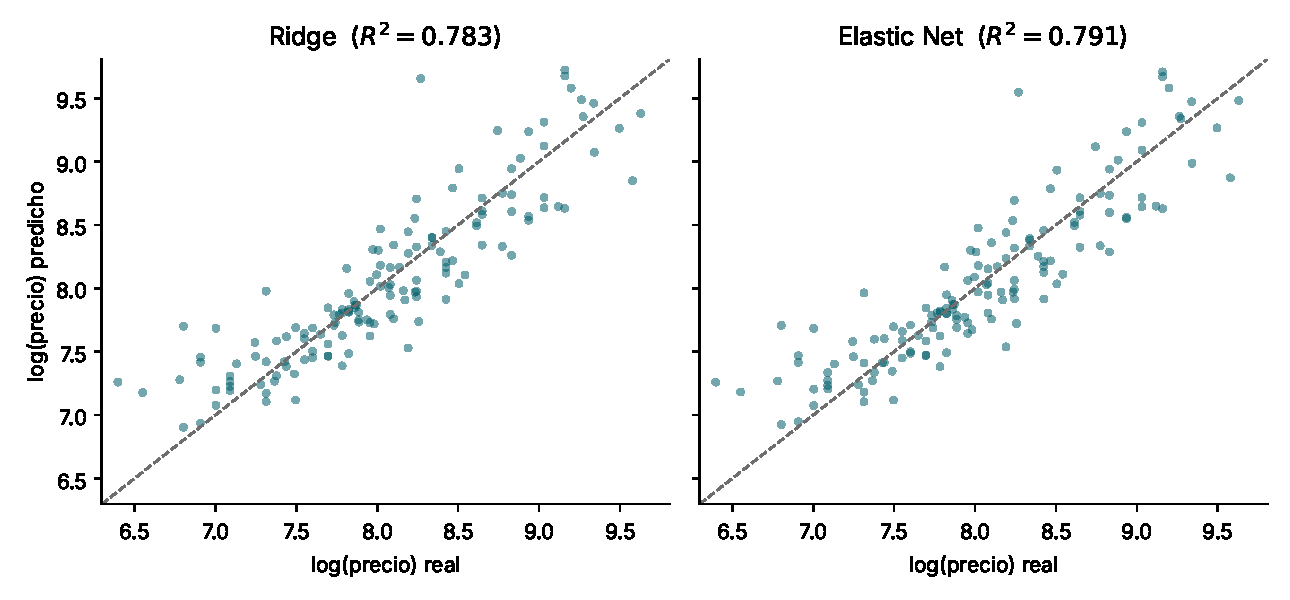
\includegraphics[width=0.95\textwidth]{figs/pred_vs_real.pdf}
\caption{Valor predicho vs. valor real de $\log(\text{precio})$ en el conjunto de prueba. La línea punteada es la identidad.}
\label{fig:pred-real}
\end{figure}

La Figura~\ref{fig:residuos} muestra los residuos de Elastic Net: se distribuyen sin un patrón sistemático alrededor de cero, aunque con un poco más de dispersión en los precios más altos, lo esperable en un mercado con outliers de lujo.

\begin{figure}[H]
\centering
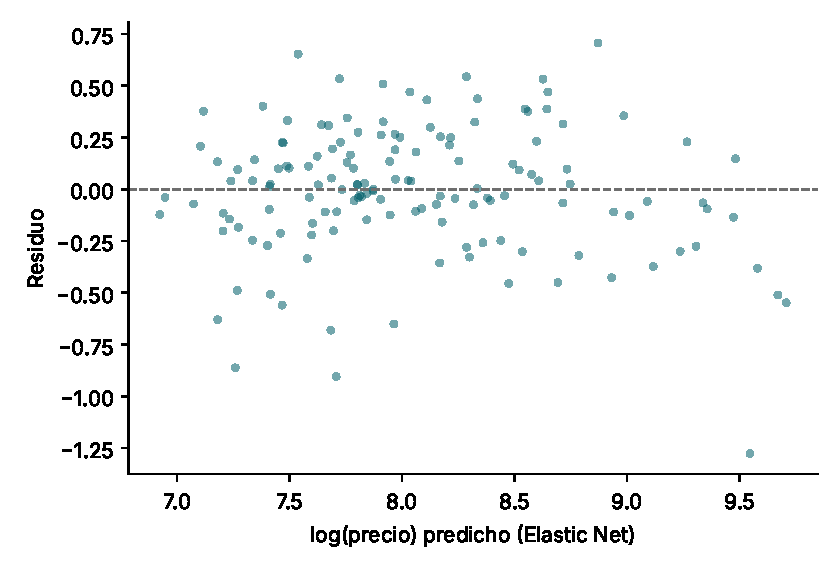
\includegraphics[width=0.62\textwidth]{figs/residuos.pdf}
\caption{Residuos de Elastic Net vs. valor predicho, en el conjunto de prueba.}
\label{fig:residuos}
\end{figure}

\subsection{Camino de regularización y selección de variables}
La Figura~\ref{fig:reg-path} muestra el camino de regularización de Elastic Net (con $\alpha=\alpha^\star=0.9$ fijo): a medida que $\lambda$ decrece desde $\lambda_{\max}$, las variables entran al modelo de forma escalonada, tal como predice la teoría (Sección~\ref{sec:en}). En el óptimo elegido por validación cruzada (línea roja), $31$ de los $34$ coeficientes son distintos de cero; las únicas tres variables eliminadas son las interacciones \texttt{area*distrito\_San Miguel}, \texttt{area*distrito\_Surquillo} y \texttt{area*distrito\_Santiago de Surco}. Esto es consistente con el \emph{efecto de agrupación} descrito en la Sección~\ref{sec:en}: esas interacciones comparten información con el efecto principal de \texttt{area\_m2} y con las variables dummy de distrito correspondientes, y el modelo prescinde de la versión redundante conservando la más informativa.

\begin{figure}[H]
\centering
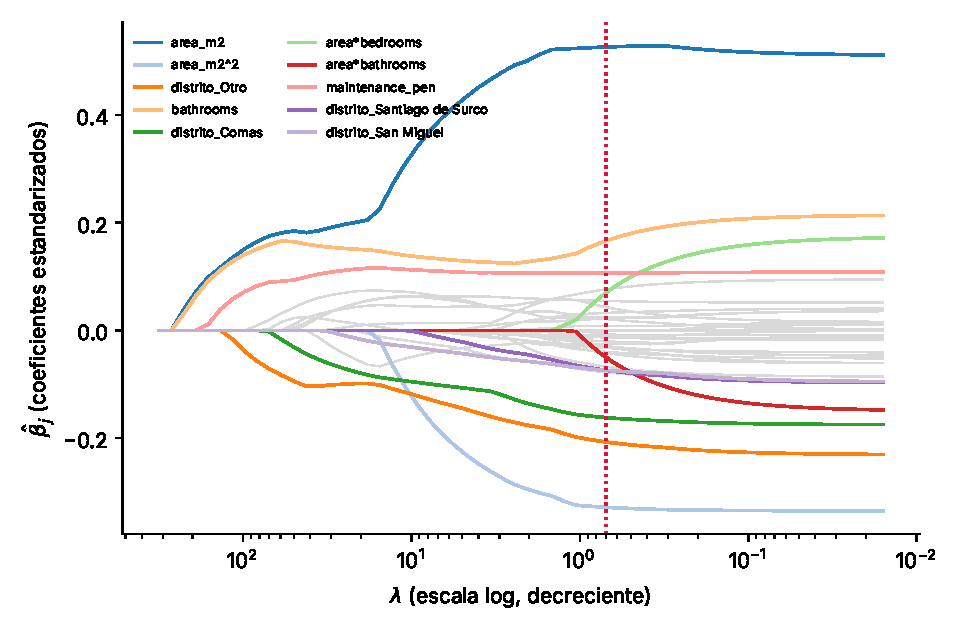
\includegraphics[width=0.78\textwidth]{figs/reg_path.pdf}
\caption{Camino de regularización de Elastic Net ($\alpha=0.9$): coeficientes estandarizados en función de $\lambda$. Se destacan las 10 variables de mayor coeficiente final; el resto se muestra en gris. La línea roja marca $\lambda^\star$.}
\label{fig:reg-path}
\end{figure}

\subsection{Verificación numérica del algoritmo}
Para confirmar que la implementación converge correctamente, la Figura~\ref{fig:convergencia} muestra $F_E(\bt_k)-F_E^\star$ en escala logarítmica durante el ajuste final de Elastic Net: el descenso por coordenadas reduce el valor de la función objetivo de forma monótona, como garantiza la Proposición~\ref{prop:convE}, y alcanza la tolerancia ($\mathrm{tol}=10^{-8}$) en $748$ ciclos.

\begin{figure}[H]
\centering
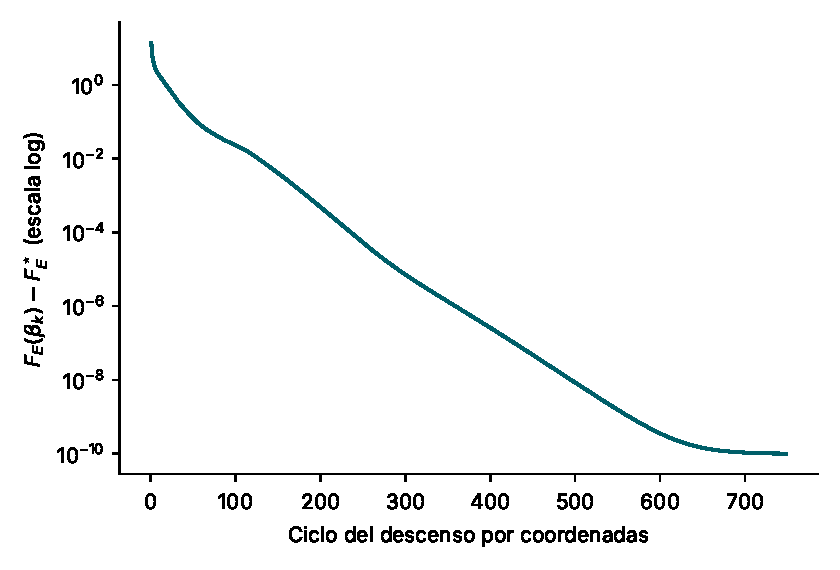
\includegraphics[width=0.62\textwidth]{figs/convergencia_en.pdf}
\caption{Convergencia del descenso por coordenadas para Elastic Net en el ajuste final.}
\label{fig:convergencia}
\end{figure}

Para Ridge, la Sección~\ref{sec:ridge} propone dos algoritmos: la solución cerrada y el descenso del gradiente (ecuación~\ref{eq:gd}). Ambos se implementaron y se corrieron sobre este mismo dataset, con $\lambda=\lambda_{\min}=1.96$ y paso $\eta=1/L$. Aquí $L=s_1^2+\lambda=3605.3$ y $\mu=s_p^2+\lambda=3.95$, de modo que $\kappa=L/\mu\approx 913$: un número de condición alto, producto de las columnas de interacción que son casi combinaciones lineales de sus componentes (Sección~\ref{sec:dataset}). Con ese $\kappa$, la Proposición~\ref{prop:gd} predice que se necesitan del orden de $\kappa\log(1/\varepsilon)$ iteraciones; en la práctica, el descenso del gradiente alcanzó la tolerancia ($\norm{\bt_{k+1}-\bt_k}<10^{-10}$) en $12\,304$ iteraciones, y su resultado final coincide con la solución cerrada con una diferencia máxima de coeficiente de $4.7\times10^{-8}$ --- muy por debajo de la cota teórica $(1-1/\kappa)^k\approx1.4\times10^{-6}$ para ese número de iteraciones. Este experimento ilustra en datos reales un punto práctico de la Sección~\ref{sec:ridge}: cuando $\kappa$ es grande, la solución cerrada (un solo sistema lineal) es muchísimo más eficiente que iterar el gradiente miles de veces; el descenso del gradiente solo es preferible cuando $p$ es tan grande que formar $X^\top X$ resulta prohibitivo.

Como verificación independiente, los tres algoritmos se compararon contra \texttt{scikit-learn} \cite{pedregosa2011}, usando la equivalencia de parámetros de la Sección~\ref{sec:sklearn} y los mismos datos estandarizados:
\begin{itemize}
\item \textbf{Ridge (solución cerrada):} diferencia máxima entre coeficientes $< 6\times10^{-15}$ (error de redondeo de punto flotante); los interceptos coinciden exactamente.
\item \textbf{Ridge (descenso del gradiente):} diferencia máxima entre coeficientes $4.7\times10^{-8}$ frente a \texttt{scikit-learn}, tras las $12\,304$ iteraciones descritas arriba.
\item \textbf{Elastic Net (descenso por coordenadas):} diferencia máxima entre coeficientes $\approx 5.6\times10^{-7}$, y la misma $R^2$ de prueba hasta el séptimo decimal.
\end{itemize}
Las tres implementaciones \emph{desde cero} --- la solución cerrada y el descenso del gradiente de Ridge, y el descenso por coordenadas de Elastic Net --- reproducen, en la práctica, la solución de referencia.

\subsection{Interpretación de los coeficientes sobre datos reales}\label{sec:interp-coef-datos}
La Tabla~\ref{tab:top-coef} muestra las variables con mayor coeficiente estandarizado en Elastic Net y su efecto porcentual aproximado sobre el precio (manteniendo las demás variables constantes), calculado como $\exp(\hat\beta_j/\sigma_j)-1$, donde $\sigma_j$ es la desviación estándar de la variable $j$ antes de estandarizar.

\begin{table}[H]
\centering
\caption{Coeficientes de mayor magnitud (Elastic Net) y su efecto aproximado sobre el precio.}\label{tab:top-coef}
\small
\begin{tabular}{@{}L{2.6cm}cL{2.5cm}L{4.6cm}@{}}
\toprule
\textbf{Variable} & $\hat\beta_j$ & \textbf{Efecto sobre el precio} & \textbf{Lectura}\\
\midrule
Área (m\textsuperscript{2}) & $0.526$ & $+0.51\,\%$ por m\textsuperscript{2} & rendimiento decreciente (ver \texttt{área\textsuperscript{2}})\\
Área\textsuperscript{2} & $-0.329$ & --- & modera el efecto del área en inmuebles grandes\\
Distrito = Otro & $-0.207$ & $-41\,\%$ & frente a Barranco (referencia), a igualdad de tamaño\\
Baños & $0.166$ & $+15.6\,\%$ por baño adicional & ---\\
Distrito = Comas & $-0.162$ & $-64\,\%$ & frente a Barranco, a igualdad de tamaño\\
Mantenimiento (S/.) & $0.107$ & $+0.03\,\%$ por sol & cuota más alta señaliza mejor edificio\\
\bottomrule
\end{tabular}
\end{table}

Dos coeficientes merecen una lectura cuidadosa porque, a primera vista, contradicen la intuición: \texttt{distrito\_La Molina} y \texttt{distrito\_Santiago de Surco} tienen coeficiente \emph{negativo} ($-0.078$ y $-0.074$), aunque ambos distritos tienen un precio \emph{promedio} más alto que la referencia (Barranco). La razón es precisamente el punto central de la regularización con variables correlacionadas: el coeficiente mide el efecto \emph{parcial} del distrito, manteniendo el área constante, y La Molina y Santiago de Surco tienen, en este dataset, el área promedio más grande de toda la muestra ($182\text{ m}^2$ y $149\text{ m}^2$) pero un precio por m\textsuperscript{2} \emph{menor} que Barranco, San Isidro o Miraflores (S/.27--30 vs. S/.36--49 por m\textsuperscript{2}). Una vez que el modelo ya atribuyó gran parte del precio al tamaño del inmueble (coeficiente de \texttt{area\_m2}), el distrito aporta un ajuste fino que, en estos dos casos, es negativo. Este resultado ilustra en datos reales exactamente lo que la Sección~\ref{sec:ridge} advierte en abstracto: en presencia de variables correlacionadas, el coeficiente de una regresión regularizada es un efecto condicional y puede tener un signo distinto al de la asociación marginal (sin controlar por las demás variables).

\subsection{Limitaciones}
El ejercicio tiene limitaciones que conviene reconocer. El tipo de cambio usado para unificar precios en soles es un valor fijo de referencia, no la tasa vigente en la fecha exacta de cada anuncio, lo que introduce un ruido adicional en los anuncios publicados en dólares. Los precios son los que pide el propietario en el anuncio (precio de oferta), no necesariamente el precio final de cierre del contrato de alquiler, que suele negociarse a la baja. El dataset solo cubre un corte de unos meses (octubre de 2022 a marzo de 2023), por lo que no permite controlar por estacionalidad ni por tendencia de precios en el tiempo. Finalmente, la limpieza del texto libre (sobre todo del año de construcción, con errores de captura evidentes) obligó a descartar una fracción de los anuncios originales, lo que puede introducir un sesgo de selección si esos anuncios no son missing completamente al azar. Ninguna de estas limitaciones invalida el ejercicio como demostración de los algoritmos y de su comportamiento teórico, pero sí matizan la interpretación de los coeficientes como estimaciones de mercado precisas.

% ==================================================================
\section{Usos actuales en el ámbito profesional}\label{sec:usos}
% ==================================================================
Ridge y Elastic Net no son solo objetos de estudio académico: son herramientas de uso diario en ámbitos donde los predictores son numerosos, están correlacionados, o $p$ es comparable (o mayor) a $n$ --- exactamente el tipo de problema reproducido en la Sección~\ref{sec:dataset}.

\textbf{Valoración automática de inmuebles (AVM).} El ejercicio de la Sección~\ref{sec:dataset} es, de hecho, una versión simplificada de los \emph{Automated Valuation Models} que usan portales inmobiliarios y bancos para tasar propiedades a partir de características estructurales y de ubicación \cite{pace2008}. Modelos como el Zestimate de Zillow combinan regresión regularizada con otros métodos para estimar el valor de millones de propiedades sin tasación manual; la selección de variables de Elastic Net es útil ahí porque el número de características de una vivienda (ubicación detallada, amenities, antigüedad, remodelaciones, comparables cercanos) crece rápido y muchas están correlacionadas, igual que en este informe.

\textbf{Econometría y modelos de precios hedónicos.} La especificación log-lineal usada en la Sección~\ref{sec:dataset} --- precio en logaritmo, predictores centrados y estandarizados --- es el estándar en economía urbana para estudiar cuánto vale cada atributo de una vivienda (localización, tamaño, antigüedad) \cite{hastie2009}. Ridge se usa cuando hay muchas variables de control correlacionadas (por ejemplo, decenas de variables de barrio) y se prioriza la estabilidad de la estimación sobre la selección de variables.

\textbf{Genómica y bioinformática.} Elastic Net es uno de los métodos más usados para relacionar la expresión de miles de genes con un fenotipo (por ejemplo, respuesta a un tratamiento o riesgo de una enfermedad), donde el número de genes ($p$) supera ampliamente al número de pacientes ($n$) y los genes de una misma vía biológica están correlacionados entre sí \cite{zou2005}. La implementación \texttt{glmnet} \cite{friedman2010}, basada en el mismo descenso por coordenadas de este informe, es un estándar de facto en bioestadística para este tipo de problema.

\textbf{Finanzas cuantitativas.} Los modelos de factores de riesgo (p. ej. modelos tipo Fama-French extendidos) suelen tener decenas de factores candidatos, muchos de ellos correlacionados entre sí; Ridge estabiliza las exposiciones estimadas y Elastic Net ayuda a seleccionar un subconjunto de factores parsimonioso para explicar los retornos de una cartera.

\textbf{Procesamiento de señales (\textit{compressed sensing}).} La penalización L1 que usa Elastic Net (y LASSO) es la base matemática de la reconstrucción de señales e imágenes a partir de mediciones incompletas, incluida la resonancia magnética acelerada en radiología \cite{beck2009}, donde se explota que la señal es dispersa en algún dominio.

\textbf{Modelos de riesgo crediticio y marketing.} Los \textit{scorecards} de crédito y los modelos de respuesta a campañas de marketing combinan frecuentemente cientos de variables correlacionadas (historial de pago, variables demográficas, transaccionales); Elastic Net se usa para obtener un modelo interpretable y con pocas variables activas, un requisito regulatorio en el caso del crédito.

% ==================================================================
\section{Conclusiones}
% ==================================================================
La regularización reemplaza el problema mal condicionado de MCO por uno convexo mejor planteado. Ridge conduce a un problema fuertemente convexo con solución cerrada y descenso del gradiente lineal. Elastic Net agrega una penalización L1 no diferenciable, que se maneja con la umbralización suave y algoritmos de primer orden como el descenso por coordenadas, y logra selección de variables con estabilidad. En ambos, $\lambda$ regula la contracción y se elige por validación cruzada; en Elastic Net, $\alpha$ regula además cuánta esparsidad se busca.

Sobre el dataset real de alquileres en Lima ($n=720$, $p=34$), las tres implementaciones \emph{desde cero} (Ridge por solución cerrada y por descenso del gradiente, y Elastic Net por descenso por coordenadas) reprodujeron la solución de \texttt{scikit-learn} con una diferencia despreciable, y Elastic Net ($R^2=0.791$ en prueba) superó tanto a Ridge como a MCO sin regularizar, seleccionando automáticamente $31$ de $34$ variables y descartando exactamente las interacciones redundantes que la teoría de la Sección~\ref{sec:en} predice que debería descartar. Los modelos estudiados son, además, piezas estándar en valoración inmobiliaria, econometría, genómica, finanzas cuantitativas y procesamiento de señales.

% ==================================================================
\begin{thebibliography}{99}

\bibitem{hoerl1970} Hoerl, A. E., \& Kennard, R. W. (1970). Ridge regression: Biased estimation for nonorthogonal problems. \emph{Technometrics}, 12(1), 55--67.

\bibitem{pace2008} Mayer, M., Bourassa, S. C., Hoesli, M., \& Scognamiglio, D. (2022). Machine learning applications to land and structure valuation. \emph{Journal of Risk and Financial Management}, 15(5), 193.

\bibitem{zou2005} Zou, H., \& Hastie, T. (2005). Regularization and variable selection via the elastic net. \emph{Journal of the Royal Statistical Society: Series B}, 67(2), 301--320.

\bibitem{hastie2009} Hastie, T., Tibshirani, R., \& Friedman, J. (2009). \emph{The Elements of Statistical Learning} (2.ª ed.). Springer.

\bibitem{beck2009} Beck, A., \& Teboulle, M. (2009). A fast iterative shrinkage-thresholding algorithm for linear inverse problems. \emph{SIAM Journal on Imaging Sciences}, 2(1), 183--202.

\bibitem{beck2017} Beck, A. (2017). \emph{First-Order Methods in Optimization}. SIAM.

\bibitem{friedman2010} Friedman, J., Hastie, T., \& Tibshirani, R. (2010). Regularization paths for generalized linear models via coordinate descent. \emph{Journal of Statistical Software}, 33(1), 1--22.

\bibitem{tseng2001} Tseng, P. (2001). Convergence of a block coordinate descent method for nondifferentiable minimization. \emph{Journal of Optimization Theory and Applications}, 109(3), 475--494.

\bibitem{pedregosa2011} Pedregosa, F., et al. (2011). Scikit-learn: Machine Learning in Python. \emph{Journal of Machine Learning Research}, 12, 2825--2830.

\end{thebibliography}

\clearpage
\begin{center}
\rule{\linewidth}{0.8pt}\\[4pt]
{\LARGE\bfseries\color{acento} Anexo --- Repositorio de C\'odigo}\\[4pt]
\rule{\linewidth}{0.8pt}
\end{center}
\vspace{6pt}

\noindent\textbf{Integrantes del grupo:}

\begin{center}
\renewcommand{\arraystretch}{1.25}
\begin{tabular}{L{9.5cm}L{3cm}}
\toprule
\textbf{Apellidos y nombres} & \textbf{C\'odigo} \\
\midrule
Cuevas S\'anchez, Jorge & 202510326 \\
Veramendi Hilario, Lando & 202210370 \\
Murillo Chancahua\~na, Jos\'e Mart\'in & 202510230 \\
Cabanillas Sol\'is, Joseph Jossemy & 202410347 \\
Honores Chiroque, Flavia Marife & 202310550 \\
\bottomrule
\end{tabular}
\end{center}

\vspace{8pt}
\noindent Todo el c\'odigo empleado para el desarrollo de este trabajo (limpieza de datos, construcci\'on de la matriz de dise\~no, implementaciones desde cero de Ridge y Elastic Net, validaci\'on cruzada, ajuste final, verificaci\'on num\'erica y generaci\'on de figuras) se encuentra disponible p\'ublicamente en el siguiente repositorio de GitHub:

\begin{center}
\colorbox{acento!8}{%
\parbox{0.92\linewidth}{\centering\vspace{3pt}
\ttfamily\color{acento}\bfseries https://github.com/Josephcpf/proyecto-optimizacion.git
\vspace{3pt}}}
\end{center}

\vspace{6pt}
\noindent\textbf{Estructura del repositorio.} La estructura de carpetas y archivos es la siguiente:

\begin{center}
\renewcommand{\arraystretch}{1.2}
\begin{tabular}{L{5.2cm}L{8.3cm}}
\toprule
\textbf{Archivo} & \textbf{Descripci\'on} \\
\midrule
\texttt{src/01\_clean.py} & Limpieza del dataset crudo de Properati Per\'u: extracci\'on de precio, dormitorios, ba\~nos, \'area, antig\"uedad, mantenimiento y distrito a partir de texto; filtrado de valores at\'ipicos y construcci\'on de \texttt{dataset\_clean.csv}. \\
\texttt{src/02\_design.py} & Construcci\'on de la matriz de dise\~no (\texttt{X\_full.csv}, $p=34$): variables num\'ericas, dummies de tipo de vivienda y distrito, interacciones y t\'erminos cuadr\'aticos; transformaci\'on logar\'itmica del precio (\texttt{y.csv}). \\
\texttt{src/models.py} & Implementaciones desde cero de \texttt{RidgeScratch} (soluci\'on cerrada) y \texttt{ElasticNetScratch} (descenso por coordenadas con umbral suave), validadas num\'ericamente contra scikit-learn. \\
\texttt{src/03\_pipeline.py} & Pipeline completo: partici\'on entrenamiento/prueba, estandarizaci\'on, validaci\'on cruzada de 5 pliegues para Ridge y Elastic Net, ajuste final, m\'etricas de desempe\~no, comparaci\'on con scikit-learn y camino de regularizaci\'on. \\
\texttt{src/04\_figuras.py} & Generaci\'on de las figuras del informe (predicho vs.\ real, curva de validaci\'on cruzada, camino de regularizaci\'on, convergencia, comparaci\'on de coeficientes, residuos). \\
\texttt{src/05\_gd\_check.py} & Verificaci\'on num\'erica del descenso del gradiente para Ridge sobre el dataset real: c\'alculo de $L$, $\mu$, $\kappa$, n\'umero de iteraciones hasta convergencia y diferencia m\'axima de coeficientes frente a la soluci\'on cerrada y a scikit-learn. \\
\texttt{data/dataset\_clean.csv} & Dataset limpio utilizado para el entrenamiento y la validaci\'on ($n=720$ observaciones, $p=34$ variables tras la construcci\'on de caracter\'isticas). \\
\texttt{figs/*.pdf} & Figuras generadas autom\'aticamente a partir de los resultados del pipeline, incluidas en este informe. \\
\texttt{informe\_v4.tex} & C\'odigo fuente \LaTeX\ de este informe. \\
\bottomrule
\end{tabular}
\end{center}

\vspace{6pt}
\noindent\textbf{Reproducibilidad.} El pipeline completo puede ejecutarse localmente instalando las dependencias necesarias y corriendo los scripts de la carpeta \texttt{src/} en orden num\'erico:

\begin{center}
\colorbox{gray!10}{%
\parbox{0.92\linewidth}{\ttfamily\small
pip install numpy pandas scikit-learn matplotlib\\[2pt]
python 01\_clean.py \&\& python 02\_design.py \&\& \textbackslash\\
python 03\_pipeline.py \&\& python 04\_figuras.py \&\& python 05\_gd\_check.py}}
\end{center}

\end{document}
